\documentclass[./main.tex]{subfiles}
\graphicspath{{\subfix{./figs}}}

% ------------ main document ------------ 
\begin{document}

\thispagestyle{empty}

% Set the line width to 1mm
\setlength{\arrayrulewidth}{0.5mm}

\begin{table}[t!]
    \centering
    \small
    %\renewcommand{\arraystretch}{1.2} % Adjust row spacing
    \begin{tabular}{ 
 >{\raggedright\raggedbottom\arraybackslash}m{1cm} 
 >{\raggedright\raggedbottom\arraybackslash}m{9cm}  
 >{\raggedright\arraybackslash}m{3cm}} % preset number of columns and aligment
         &  \DocCredential & \textbf{\DocId} \\
        \hline 
        & & \\
        & \vspace{2.5mm} \Large \textbf{\DocField} & \\ [4mm]        
        & \scriptsize \sf \MakeUppercase \DocType & \\ [4mm]
        & \large \textbf{\DocTitle}  & \textbf{Version \DocVersion}  \\ [8mm]
        & \DocSubtitle &  Porto Alegre,\newline \DocDate\\ [10mm]
        \multicolumn{3}{p{12cm}}{\scriptsize \DocComment} \\
        \hline
    \end{tabular}
\end{table}

\normalsize

\begin{center}
    \large
    \textbf{Abstract}
\end{center}

\noindent \DocAbs


\noindent \textbf{keywords} --- \DocKWA; \DocKWB; \DocKWC.
    \newline
    \newline
    \newline
    \noindent \textbf{highlights}:
        \small
        \begin{enumerate}
            \item \DocHLA; 
            \item \DocHLB;
            \item \DocHLC.
        \end{enumerate}

\clearpage

% --------------- Graphical Abstract ---------------
\begin{center}
    \large \textbf{Graphical abstract}
\end{center}        
\vspace{5mm}
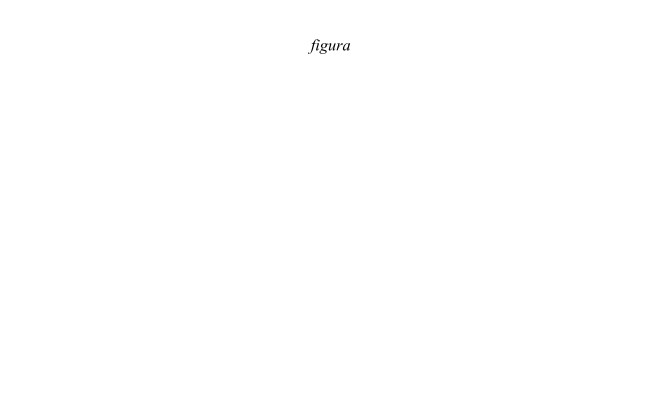
\includegraphics[width=\textwidth]{figs/gabs.jpg}
\clearpage

\end{document}